% System
\section{System: \textsc{PRDWeaver}}
\label{sec:system}

\textsc{PRDWeaver} is a modular, multi-agent pipeline that generates a schema-conformant PRD from a brief.
The orchestrator routes intermediate artifacts between agents, and a final assembler produces the output PRD.

\begin{figure}[t]
  \centering
  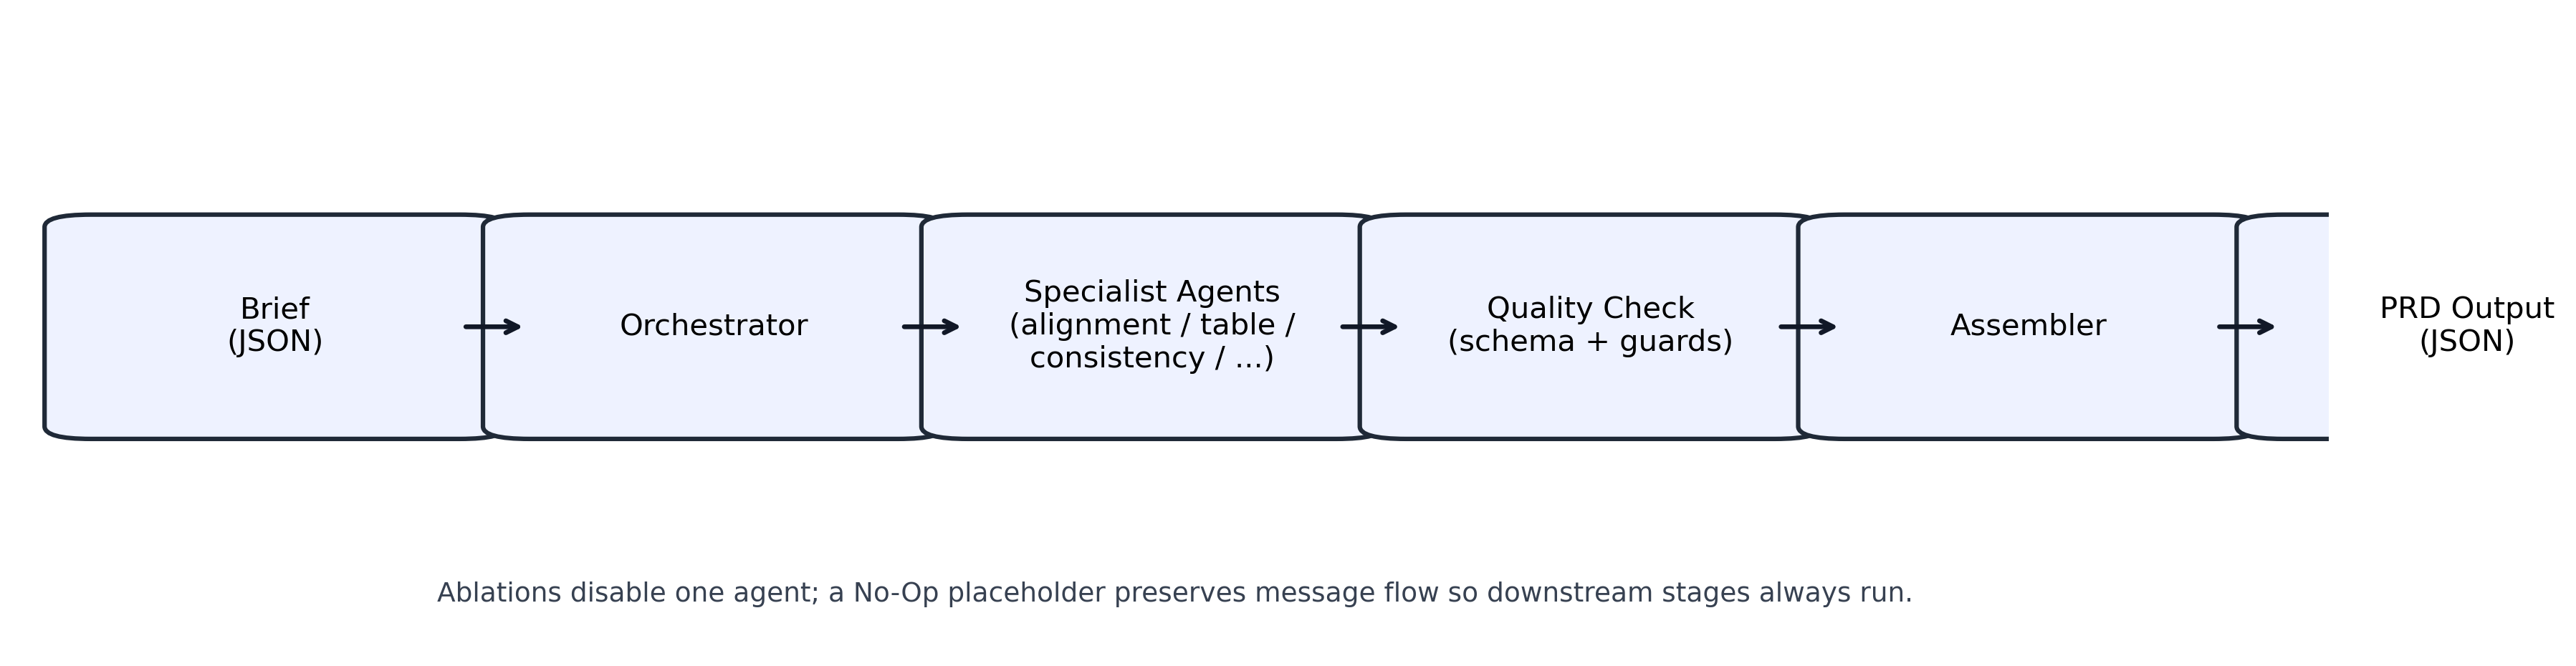
\includegraphics[width=\columnwidth]{figures/framework_pipeline.png}
  \caption{System overview. \textsc{PRDWeaver} orchestrates specialist agents and assembles a schema-conformant PRD. In ablations, disabled agents are replaced by a no-op placeholder to preserve message flow.}
  \label{fig:framework}
\end{figure}

\paragraph{Agents.}
We use specialized agents for complementary roles, including:
(i) an alignment agent to restate goals and constraints,
(ii) optional vision/table agents to structure content into tables/figures when applicable,
(iii) a consistency agent to enforce terminology and section-to-section coherence,
and (iv) a quality/verification stage that validates schema completeness prior to assembly.

\paragraph{Ablation-ready design.}
To enable controlled ablations, disabled agents are replaced with a no-op placeholder that preserves message flow.
This prevents pipeline breaks and ensures that downstream stages (quality checks and assembly) always run, making ablation outputs directly comparable.

\paragraph{Outputs.}
The final PRD is serialized as JSON under a fixed schema and can be exported into human-readable formats (e.g., DOCX) for inspection.


